\begin{frame}
    \frametitle{Introduction}
    \framesubtitle{Motivation}

    \begin{columns}
        \begin{column}{0.6\textwidth}
            \begin{itemize}
                \item Dynamical evolution of a dense stellar systems.
                      ({\nbody} Problem)
                \item Newtonian systems compounded by \blue{more than two stars},
                      needs numerical approaches.
                \item Evolution of the High Performance Computing (HPC).
            \end{itemize}
        \end{column}
        \begin{column}{0.4\textwidth}
            \begin{figure}
                \centering
                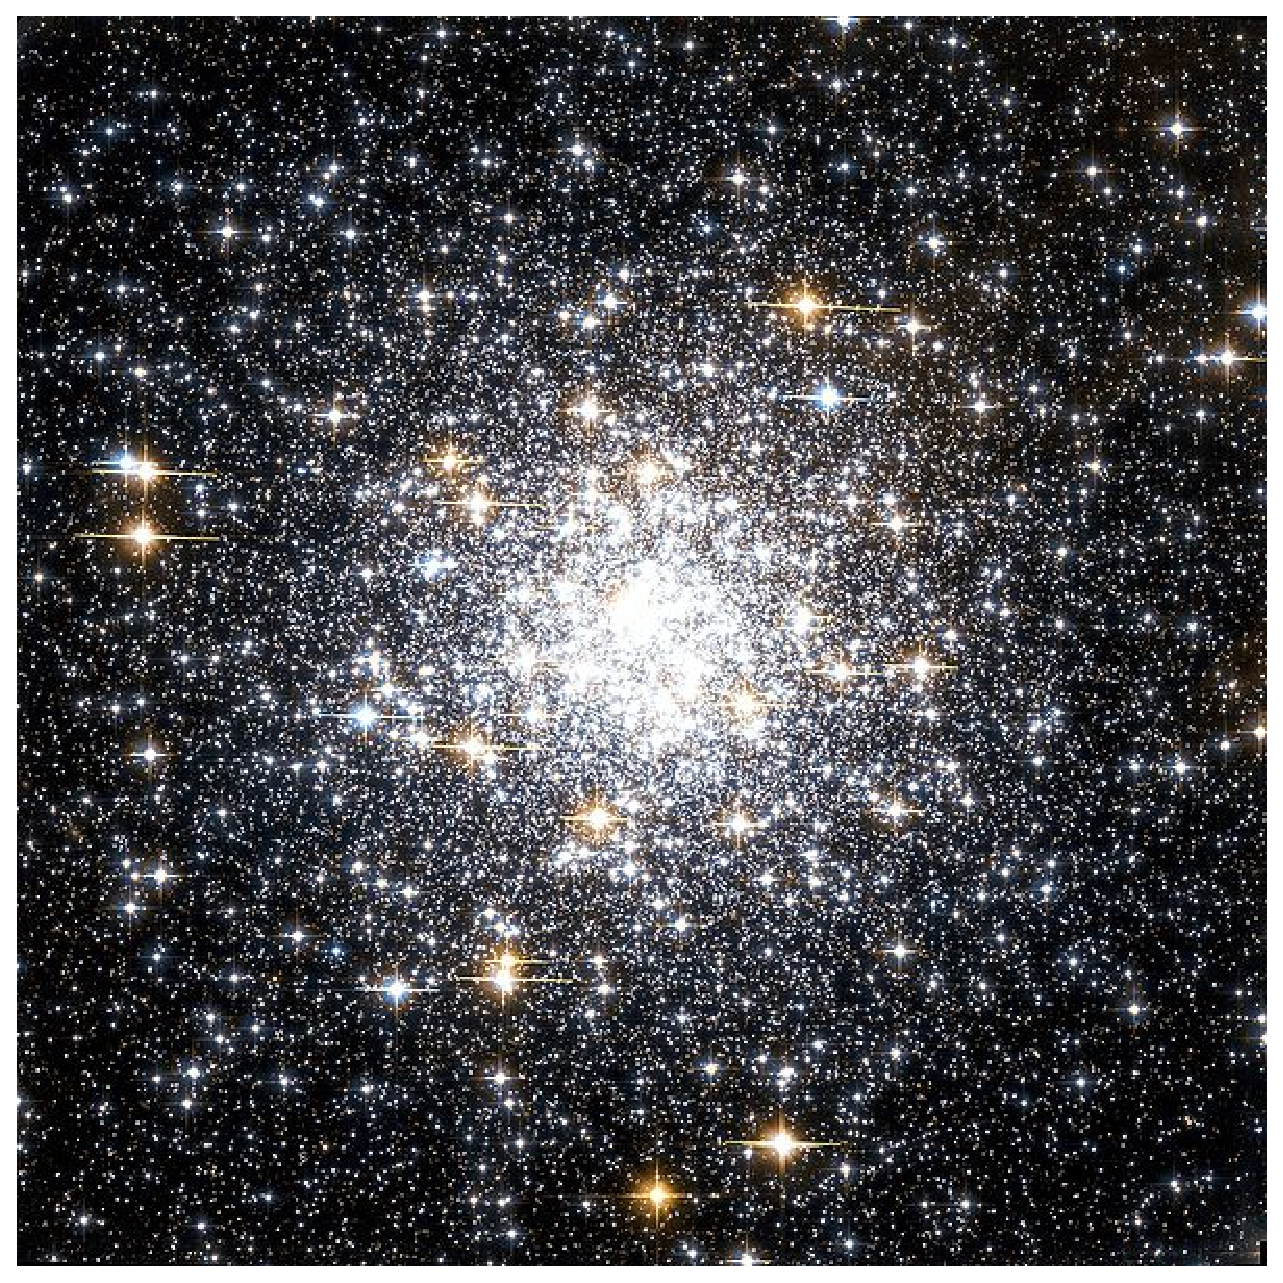
\includegraphics[width=0.8\textwidth]{img/m69}
                \caption{Globular cluster ``Messier 69'' in the constellation Sagittarius.}
                \label{fig:m69}
            \end{figure}
        \end{column}
    \end{columns}

\end{frame}

\begin{frame}
    \frametitle{Introduction}
    \framesubtitle{{\nbody} algorithms classification}

    \begin{description}
        \item[Collision-less]
            A star just sees the \blue{background potential} of the rest of
            the stellar system.
            A model of this situation is the Barnes-Hut Treecode
            with a complexity $O(N\log N)$~\cite{BarnesHut86}
            or the fast multipole method with $O(N)$~\cite{GreendardThesis}.
            \vspace{0.7cm}
        \item[Collisional (``direct-summation'')]
            One star integrates \blue{all gravitational forces}
            for all stars. This typically scale as $O(N^{2})$.
            A well-known example is the family of algorithm of Aarseth
            the direct-summation {\sc Nbody} integrator~\cite{Aarseth99,Spurzem1999,Aarseth03}
            or {\sc kira} code~\cite{PortegiesZwartEtAl01}.
    \end{description}

\end{frame}


\begin{frame}
    \frametitle{Introduction}
    \framesubtitle{The computational challenge}

    \begin{itemize}
        \item The {\nbody} codes evolution is related to the available
                \blue{hardware} in our time.
        \item The algorithms with a complexity of $O(N^{2})$ require
                \red{supercomputers}.
        \begin{itemize}
            \item  e.g \blue{beowulf clusters},
                which require a parallelization of the code
                ({\sc Nbody6++} developed by Spurzem et al.~\cite{Spurzem1999}).

            \item Special-purpose hardware, like the \blue{GRAPE} (short for GRAvity
                PipE system~\cite{TMFES96,MT98,Makino98,GRAPE6A}.

        \end{itemize}

        \item  The literature overview reveals a strong interest on porting the existing codes to the
            \blue{GPU} architecture, like e.g. the work
            of~\cite{Portegies2007a,Hamada2007,Belleman2008}
            on single nodes or using large
            clusters~\cite{berczik2011high,NitadoriAarseth2012,Capuzzo-DolcettaEtAl2013}.

    \end{itemize}

\end{frame}
